\documentclass[11pt,oneside,a4paper,final]{article}

\usepackage{ifpdf}
%HEVEA\pdffalse

\ifpdf
\usepackage{fancyhdr}
\usepackage{lastpage}

\pagestyle{fancy}

\renewcommand{\headrulewidth}{0.0pt}

\lhead{}
\chead{}
\rhead{}
\lfoot{}
\cfoot{Page {\thepage} of \pageref{LastPage}}
\rfoot{}
\fi

\usepackage{longtable}

\usepackage[T1]{fontenc}  
\usepackage{textcomp}  
\usepackage{lmodern}  

% \usepackage[style=numeric,backend=biber]{biblatex}
% \usepackage[style=numeric]{biblatex}
\bibliography{programmer_guide}
% \usepackage[hidelinks=true]{hyperref}



\usepackage{hyperref}

\hypersetup{  
  colorlinks=true,
  final=true,
  pdftitle="gVirtualXRay - Tutorial 02 - GLUT",
  pdfauthor="Dr Franck P. Vidal",  
  pdfsubject="Loading the shader program from a file compressed with the Z library. 
		Adding an efficient mouse control to turn the 3D scene."
}

\usepackage[paper=a4paper,margin=1.6cm]{geometry}	% 1 inch margins all around

\usepackage[british=nohyphenation]{hyphsubst}


\usepackage[british]{babel}
\usepackage{graphicx}
\usepackage[font=normalsize,labelfont=sf,textfont=sf]{subfig}
\captionsetup*[subfigure]{position=bottom}
\usepackage{color}

\definecolor{mygreen}{rgb}{0,0.6,0}
\definecolor{mygray}{rgb}{0.5,0.5,0.5}
\definecolor{mymauve}{rgb}{0.58,0,0.82}

\usepackage{listings}
 \lstset{ %
  literate={"}{\textquotedbl}1,
  backgroundcolor=\color{white},   % choose the background color; you must add \usepackage{color} or \usepackage{xcolor}
  basicstyle=\footnotesize,        % the size of the fonts that are used for the code
  breakatwhitespace=false,         % sets if automatic breaks should only happen at whitespace
  breaklines=true,                 % sets automatic line breaking
  captionpos=b,                    % sets the caption-position to bottom
  commentstyle=\color{mygreen},    % comment style
%   deletekeywords={...},            % if you want to delete keywords from the given language
%   escapeinside={\%*}{*)},          % if you want to add LaTeX within your code
  extendedchars=true,              % lets you use non-ASCII characters; for 8-bits encodings only, does not work with UTF-8
  frame=single,                    % adds a frame around the code
  keepspaces=true,                 % keeps spaces in text, useful for keeping indentation of code (possibly needs columns=flexible)
  keywordstyle=\color{blue},       % keyword style
  language=C++,                 % the language of the code
%   morekeywords={*,...},            % if you want to add more keywords to the set
  numbers=left,                    % where to put the line-numbers; possible values are (none, left, right)
  numbersep=5pt,                   % how far the line-numbers are from the code
  numberstyle=\tiny\color{mygray}, % the style that is used for the line-numbers
  rulecolor=\color{black},         % if not set, the frame-color may be changed on line-breaks within not-black text (e.g. comments (green here))
  showspaces=false,                % show spaces everywhere adding particular underscores; it overrides 'showstringspaces'
  showstringspaces=false,          % underline spaces within strings only
  showtabs=false,                  % show tabs within strings adding particular underscores
  stepnumber=1,                    % the step between two line-numbers. If it's 1, each line will be numbered
  stringstyle=\color{mymauve},     % string literal style
  tabsize=2,                       % sets default tabsize to 2 spaces
  title=\lstname                   % show the filename of files included with \lstinputlisting; also try caption instead of title
}

% \usepackage[acronym,toc]{glossaries}
% \makeglossaries
% % \phantomsection
% \addcontentsline{toc}{section}{Acronyms}
% \section*{Acronyms}
% \begin{footnotesize}
% \begin{acronym}[TDMA]

% \newacronym{2D}{2D}{two-dimensional}
\newacronym{3D}{3D}{three-dimensional}
\newacronym{FBO}{FBO}{frame buffer object}
\newacronym{FLTK}{FLTK}{Fast Light Toolkit}
\newacronym{GLEW}{GLEW}{OpenGL Extension Wrangler Library}
\newacronym{GLSL}{GLSL}{OpenGL Shading Language}
\newacronym{GLU}{GLU}{OpenGL Utility Library}
\newacronym{GLUT}{GLUT}{OpenGL Utility Toolkit}
\newacronym{GPU}{GPU}{Graphics Processor Unit}
% \newacronym{GUI}{GUI}{graphical user interface}
% \newacronym{Gzip}{Gzip}{GNU zip}
% \newacronym{ITK}{ITK}{Insight Segmentation and Registration Toolkit}
\newacronym{keV}{keV}{kiloelectron volt}
% \newacronym{MXE}{MXE}{M cross environment}
\newacronym{STL}{STL}{STereoLithography}
\newacronym{SVN}{SVN}{Subversion}
\newacronym{VBO}{VBO}{vertex buffer object}
% \newacronym{VTK}{VTK}{Visualization Toolkit}
% 


\title{gVirtualXRay -- Tutorial 02 -- GLUT: \\
		Loading the shader program from a file compressed with the Z library.\\
		Adding an efficient mouse control to turn the 3D scene.}

\author{Dr Franck P. Vidal}
\date{27\textsuperscript{th} September 2014}

\begin{document}
 \sloppy

\maketitle
\vfill
\begin{center}
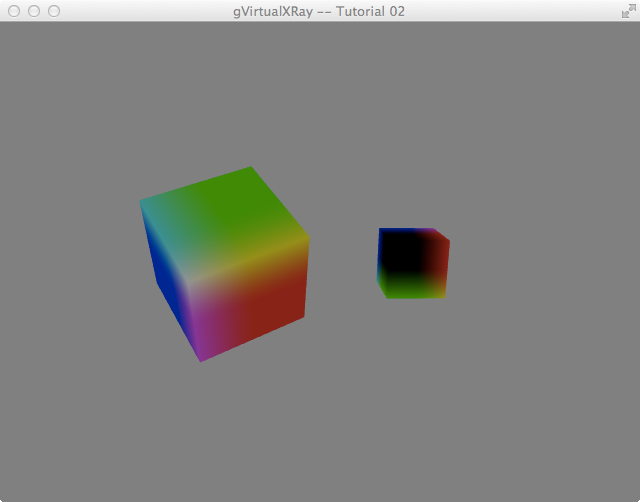
\includegraphics[width=0.5\textwidth]{screenshot}
\end{center}
\vfill


 \newpage
\phantomsection
\addcontentsline{toc}{section}{Table of contents}
\tableofcontents

\ifpdf
\newpage
\phantomsection
\addcontentsline{toc}{section}{List of figures}
\listoffigures

% \newpage
% \phantomsection
% \addcontentsline{toc}{section}{List of tables}
% \listoftables

% \newpage
\phantomsection
\addcontentsline{toc}{section}{List of listings}
\lstlistoflistings
\fi

\newpage


%%%%%%%%%%%%%%%%%%%%%%%%%%%%%%%%%%%%%%%%%%%%%%%%%%%%%%%%%%%%%%%%%%%%%%%%%%%%%%%%
\section{Introduction}

The complete source code of this tutorial is available in 
Appendix~\ref{sec:Program Source Code} and on the Subversion (SVN) repository 
at 
\verb+tutorials/tutorial_02_glut/tutorial_02_glut.cxx+. 
It can be downloaded here: 
\url{
https://sourceforge.net/p/gvirtualxray/code/HEAD/tree/trunk/tutorials/tutorial_02_glut/tutorial_02_glut.cxx}.
It improves the 1st tutorial in two ways:
\begin{enumerate}
	\item Loading the shader program from a file compressed with the Z library.
	\item Adding an efficient mouse control to turn the 3D scene.
\end{enumerate}
Two cubes are displayed (see Figure~\ref{fig:scene}). 
\begin{figure}[bth]
 \centering
 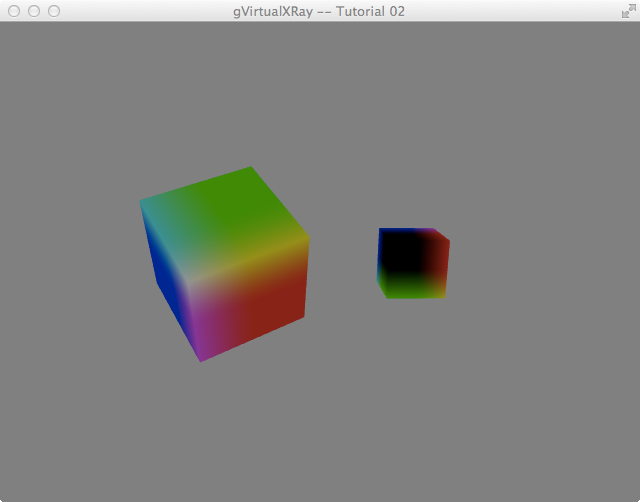
\includegraphics[width=0.5\textwidth]{screenshot}
 \caption{\label{fig:scene} Screen capture of the second tutorial.}
\end{figure}
First the fragment program is saved into \verb+tutorial_02_gl2.frag+. 
The vertex program is saved into \verb+tutorial_02_gl2.vert+. 
Our implementation supports OpenGL 2.x only when GLUT is used. 
OpenGL 3.x and OpenGL 4.x or above are supported when GLFW is used. 
The files are individually compressed using \textit{gzip}\,\footnote{\url{http://www.gzip.org/}}. 
Finally each compressed file is converted into a C header file. 
It can be achieved CMake\,\footnote{\url{http://www.cmake.org/}} or an external tool such as bin2c\,\footnote{\url{http://sourceforge.net/projects/bin2c/}}. 

The tutorial is organised as follows:
\begin{itemize}
 \item Section~\ref{sec:Header inclusion} shows the header files to include. 

 \item Section~\ref{sec:Name Spaces} shows some of the name spaces that can be 
	included to lighten the code. 
	% How to set up all the main components of the simulation is describe in 

 \item Section~\ref{sec:Global Variables} shows the global variables that are 
	used. 

 \item Section~\ref{sec:Function Declarations} what functions have to 
	be declared. 

 \item Section~\ref{sec:Initialise Shaders} shows how to initialise the shaders from compressed data stored in C header files. 

 \item Section~\ref{mouseButtonCallback} shows the callback for mouse button events. 
 The mouse is used to rotate objects in an intuitive way. 

 \item Section~\ref{cursorPosCallback} shows how callback for cursor position events works. 

 \item How to convert screen coordinates to arcball vectors is explained in Section~\ref{getArcballVector} 

 \item The conversion from radian to degree is shown in Section~\ref{radian2degree}.

 \item Section~\ref{computeRotation} shows how the corresponding rotation matrix is computed. 
 
 \item Section~\ref{sec:Next Tutorial} gives a preview of what the next 
  tutorial will be about.
 
 \item Appendix~\ref{sec:Program Source Code} shows the source code of this 
	tutorial. 
		
\end{itemize}


%%%%%%%%%%%%%%%%%%%%%%%%%%%%%%%%%%%%%%%%%%%%%%%%%%%%%%%%%%%%%%%%%%%%%%%%%%%%%%%%
\section{Header inclusion}
\label{sec:Header inclusion}

Listing~\ref{lst:header} only shows the new i) the macros that have to be defines to include 
OpenGL core profile headers and ii) the header files that need to be included to decompress the data using the \textbf{zlib} library\,\footnote{\url{http://www.zlib.net/}}:
\begin{itemize}
 \item \verb+gVirtualXRay/Utilities.h+ is the new header file that is used to handle decompression using the Z library. 
 \item \verb+tutorial_02_gl2.frag.h+ is the compressed fragment shader for OpenGL 2.x. 
 \item \verb+tutorial_02_gl2.vert.h+ is the compressed vertex shader for OpenGL 2.x. 
% \item \verb+tutorial_02_gl3.frag.h+ is the compressed fragment shader for OpenGL 3.x or OpenGL 4.x. 
% \item \verb+tutorial_02_gl3.vert.h+ is the compressed vertex shader for OpenGL 3.x or OpenGL 4.x. 
 \item For other header files, see the GLUT version of Tutorial 1.
\end{itemize}

\begin{center}
\lstinputlisting[firstline=65, lastline=100, caption=Header inclusion., 
label=lst:header]{../../../tutorials/tutorial_02_glut/tutorial_02_glut.cxx}
\end{center}


%%%%%%%%%%%%%%%%%%%%%%%%%%%%%%%%%%%%%%%%%%%%%%%%%%%%%%%%%%%%%%%%%%%%%%%%%%%%%%%%
\section{Name Spaces}
\label{sec:Name Spaces}

See Tutorial 1.


%%%%%%%%%%%%%%%%%%%%%%%%%%%%%%%%%%%%%%%%%%%%%%%%%%%%%%%%%%%%%%%%%%%%%%%%%%%%%%%%
\section{Global Variables}
\label{sec:Global Variables}

Listing~\ref{lst:global variables} shows the global variables that are used:
\begin{itemize}

 \item \verb+g_rotation_speed+ controls the speed of rotation  of the cubes. 

 \item \verb+g_tutorial_02_gl2_frag+  is declared in \verb+tutorial_02_gl2.frag.h+. 
 It is the compressed fragment shader for OpenGL 2.x.
 
 \item \verb+g_tutorial_02_gl2_vert+  is declared in \verb+tutorial_02_gl2.vert.h+. 
 It is the compressed vertex shader for OpenGL 2.x.

% \item \verb+g_tutorial_02_gl3_frag+  is declared in \verb+tutorial_02_gl3.frag.h+. 
% It is the compressed fragment shader for OpenGL 3.x or OpenGL 4.x.
% 
% \item \verb+g_tutorial_02_gl3_vert+  is declared in \verb+tutorial_02_gl3.vert.h+. 
% It is the compressed vertex shader for OpenGL 3.x or OpenGL 4.x.

\item \verb+bool g_use_arc_ball+ is used to know if arc ball rotation is currently in use.

\item \verb+int g_button+ stores which button generated an event last.

\item \verb+int g_button_state+ stores the new state of this button.

\item \verb+GLint g_last_x_position+ is the previous last known X position of the cursor.

\item \verb+GLint g_last_y_position+ is the previous last known Y position of the cursor.

\item \verb+GLint g_current_x_position+ is the current X position of the cursor.

\item \verb+GLint g_current_y_position+ is the current Y position of the cursor.

	 \item For other global variables, see the GLUT version of Tutorial 1.
\end{itemize}


\begin{center}
\lstinputlisting[firstline=110,lastline=157, caption=Global variables., 
label=lst:global variables]{../../../tutorials/tutorial_02_glut/tutorial_02_glut.cxx}
\end{center}


%%%%%%%%%%%%%%%%%%%%%%%%%%%%%%%%%%%%%%%%%%%%%%%%%%%%%%%%%%%%%%%%%%%%%%%%%%%%%%%%
\section{Function Declarations}
\label{sec:Function Declarations}

One function has been added to load shaders from compressed files and five functions have been add to control the rotation using the mouse: 
\begin{itemize}
 \item \verb+initShader+ is used i) to decompress the shaders, and ii) to compile the shaders (see Section~\ref{sec:Initialise Shaders}).

 \item \verb+mouseButtonCallback+ is called when a mouse button event occurs (see Section~\ref{mouseButtonCallback}).

 \item \verb+cursorPosCallback+ is used when the mouse moves (see Section~\ref{cursorPosCallback}).
 
  \item \verb+getArcballVector+ computes the arc ball vector given screen coordinates (see Section~\ref{getArcballVector}). 
  Details about arc ball rotation can be found at \url{http://en.wikibooks.org/wiki/OpenGL_Programming/Modern_OpenGL_Tutorial_Arcball} and \url{http://nehe.gamedev.net/tutorial/arcball_rotation/19003/}. 
 
 \item \verb+radian2degree+ converts an angle value in radians into degrees (see Section~\ref{radian2degree}).

 \item \verb+computeRotation+ generates the corresponding matrix rotation (see Section~\ref{computeRotation}).
\end{itemize}
Listing~\ref{lst:function declarations} shows the declaration of all the functions. 

\begin{center}
\lstinputlisting[firstline=160, lastline=177, caption=Function declarations., 
label=lst:function declarations]{../../../tutorials/tutorial_02_glut/tutorial_02_glut.cxx}
\end{center}


%%%%%%%%%%%%%%%%%%%%%%%%%%%%%%%%%%%%%%%%%%%%%%%%%%%%%%%%%%%%%%%%%%%%%%%%%%%%%%%%
\section{Shader Initialisation}
\label{sec:Initialise Shaders}

\begin{itemize}
\item \verb+g_display_shader+ is the instance of the Shader class that will store our GLSL programs. 

\item \verb+g_tutorial_02_gl3_vert+  is declared in \verb+tutorial_02_gl3.vert.h+. 
 It is the compressed vertex shader for OpenGL 3.x or OpenGL 4.x. 
 To generate the file, the text file containing our vertex shader was compressed using Gzip. 
 A C header was then generated from the compressed file. 
 It can be done using bin2c or CMake. 
 There is no need to distribute text files with the executable file that reads the code at runtime. 
 The code of the shader is embedded in the executable file. 

\item  The same is done for the fragment shader.  
\verb+g_tutorial_02_gl2_frag+  is declared in \verb+tutorial_02_gl2.frag.h+. 
 It is the compressed fragment shader for OpenGL 3.x or OpenGL 4.x.

\item \verb+g_tutorial_02_gl3_vert+ is decompressed into \verb+p_vertex_shader+, 
\verb+g_tutorial_02_gl3_frag+ into \verb+p_fragment_shader+, using the \verb+inflate+ function that will invoke Z library. 

\item Error codes are stored in \verb+z_lib_return_code_vertex+ and \verb+z_lib_return_code_fragment+. 
They are used to make sure the decompression has been successful. 

\item The source of the shaders are then saved into two separate \verb+std::string+ instances (\verb+vertex_shader+ and \verb+fragment_shader+). 

\item If a decompression error occurred, an exception is thrown. 

\item To help debugging, it is possible to give the vertex and fragment programs labels: 
\verb+g_display_shader.setLabels("display.vert", "display.frag")+. 

\item Finally, the Shader instance \verb+g_display_shader+ loads the source code. 
\end{itemize}
Listing~\ref{lst:Initialise Shaders} shows how to perform all these steps.
\begin{center}
\lstinputlisting[firstline=272, lastline=302, caption=Shader initialisation., 
label=lst:Initialise Shaders]{../../../tutorials/tutorial_02_glut/tutorial_02_glut.cxx}
\end{center}


%%%%%%%%%%%%%%%%%%%%%%%%%%%%%%%%%%%%%%%%%%%%%%%%%%%%%%%%%%%%%%%%%%%%%%%%%%%%%%%%
\section{Callback for Mouse Button Events}
\label{mouseButtonCallback}

This callback stores the mouse states in global variables, i.e.~which button generated an event, the type of events and the cursor's position in screen coordinates) (see Listing~\ref{lst:mouseButtonCallback}).
If the mouse button is pressed, then arcball rotation is in used. 
If the mouse button is released, then arcball rotation is stopped.

In \verb+void initGLUT()+, the callback is registered as follows:
\verb+glutMouseFunc(mouseButtonCallback)+.

\begin{center}
\lstinputlisting[firstline=529, lastline=585, caption=Callback for mouse button events., 
label=lst:mouseButtonCallback]{../../../tutorials/tutorial_02_glut/tutorial_02_glut.cxx}
\end{center}


%%%%%%%%%%%%%%%%%%%%%%%%%%%%%%%%%%%%%%%%%%%%%%%%%%%%%%%%%%%%%%%%%%%%%%%%%%%%%%%%
\section{Callback for Cursor Position Events}
\label{cursorPosCallback}

Listing~\ref{lst:cursorPosCallback} shows i) how to store the cursor's position in global variables,and ii) 
how the matrix rotation is updated accordingly.

In \verb+void initGLUT()+, the callback is registered as follows:
\verb+glutMotionFunc(cursorPosCallback)+.

\begin{center}
\lstinputlisting[firstline=588, lastline=599, caption=Callback for cursor position events., 
label=lst:cursorPosCallback]{../../../tutorials/tutorial_02_glut/tutorial_02_glut.cxx}
\end{center}


%%%%%%%%%%%%%%%%%%%%%%%%%%%%%%%%%%%%%%%%%%%%%%%%%%%%%%%%%%%%%%%%%%%%%%%%%%%%%%%%
\section{Conversion from Screen Coordinates to Arcball Vector}
\label{getArcballVector}

   Listing~\ref{lst:getArcballVector} shows how to compute the arc ball vector given screen coordinates. 
   Arcball rotation allows the user to rotate objects in a natural and intuitive way. 
  Details about arc ball rotation can be found at \url{http://en.wikibooks.org/wiki/OpenGL_Programming/Modern_OpenGL_Tutorial_Arcball} and \url{http://nehe.gamedev.net/tutorial/arcball_rotation/19003/}. 

\begin{center}
\lstinputlisting[label=lst:getArcballVector,
    firstline=602, lastline=623, 
    caption=Conversion from screen coordinates to arc ball vector.]{../../../tutorials/tutorial_02_glut/tutorial_02_glut.cxx}
\end{center}


%%%%%%%%%%%%%%%%%%%%%%%%%%%%%%%%%%%%%%%%%%%%%%%%%%%%%%%%%%%%%%%%%%%%%%%%%%%%%%%%
\section{Radian to Degree Conversion}
\label{radian2degree}

$\pi$ radians corresponds to 180~degrees. 
Listing~\ref{lst:radian2degree} shows how to perform this simple conversion. 

\begin{center}
\lstinputlisting[label=lst:radian2degree,
    firstline=626, lastline=631,
    caption=Convert an angle value from radian to degree.]{../../../tutorials/tutorial_02_glut/tutorial_02_glut.cxx}
\end{center}


%%%%%%%%%%%%%%%%%%%%%%%%%%%%%%%%%%%%%%%%%%%%%%%%%%%%%%%%%%%%%%%%%%%%%%%%%%%%%%%%
\section{Compute Rotation Matrix}
\label{computeRotation}

If the arcball rotation is currently in used, if the cursor's position has changed, then the rotation matrix is updated using the arcball technique
(see Listing~\ref{lst:computeRotation}). 

\begin{center}
\lstinputlisting[firstline=634, lastline=662, caption=Compute the arcball rotation., 
label=lst:computeRotation]{../../../tutorials/tutorial_02_glut/tutorial_02_glut.cxx}
\end{center}

	
%%%%%%%%%%%%%%%%%%%%%%%%%%%%%%%%%%%%%%%%%%%%%%%%%%%%%%%%%%%%%%%%%%%%%%%%%%%%%%%%
\section{Next Tutorial...}
\label{sec:Next Tutorial}

In the next tutorial:
\begin{itemize}
	\item Display two cubes with a better shader program and with transparency (one of the cubes is within the other one). 
	Do you see where we are going?
	
	\item Display the cubes in wireframe.
	
	\item Compute the X-ray attenuation of the cubes.
\end{itemize}


% % \newpage
% \printglossary[type=\acronymtype] 


%%%%%%%%%%%%%%%%%%%%%%%%%%%%%%%%%%%%%%%%%%%%%%%%%%%%%%%%%%%%%%%%%%%%%%%%%%%%%%%%
\appendix
\section{Program Source Code}
\label{sec:Program Source Code}

\begin{center}
  \lstinputlisting[caption=All the source code of this tutorial., 
  label=lst:Program Source Code,numbers=none]{../../../tutorials/tutorial_02_glut/tutorial_02_glut.cxx}
\end{center}

% 
% \newpage
% \phantomsection
% \addcontentsline{toc}{section}{References}
% \printbibliography
% 

\end{document}
